\documentclass[11pt]{article}



\usepackage[latin1]{inputenc}    
\usepackage[T1]{fontenc}
\usepackage[francais]{babel}     
\usepackage{listings}
\usepackage[margin=2.5cm]{geometry}
\usepackage{graphicx}

\date{INSA Lyon}
\title{Analyse de logs apache - Document de Conception}
\author{Aymeric Cousaert et Mael Risbourg}

\begin{document}
\maketitle

\vspace{1cm}
\tableofcontents
\vspace{3cm}

\begin{section}{Spécifications de l'application}
L'outil analog est un programme qui permet d'analyser un journal de logs apache.

Afin de réaliser notre projet, nous avons du réfléchir aux différents cas d'exécution nous pouvions rencontrer. Nous avons donc spécifié ces cas que nous pouvons classer en trois catégories.
 \newline
 
Premièrement, il y a les cas normaux, ceux pour lesquels le programme ne produit pas d'erreurs. Avec un bon manuel d'utilisation, ce sont ceux qui doivent arriver le plus fréquemment. Ici, nous considérons que la syntaxe des commandes est toujours correctement respectée. Par défaut, seul le nom du journal de logs (extension .log ou .txt) est donné en paramètre et notre programme affiche les 10 sites les plus consultés. Pour les autres cas énumérés ensuite, on considère que le journal de logs est le dernier paramètre fourni. 
Première possibilité, une option est rajoutée en paramètre. Notre programme affichera toujours le classement des dix sites les plus visités ; mais 
\begin{itemize}
\item parmi les documents qui ne sont pas un format image, css ou javascript si l'option -e est indiquée ;
\item parmi ceux qui ont été consultés dans l'intervalle de temps [heure;  heure  + 1[ si l'option -t heure est indiquée ;
\item un fichier .dot au format GraphViz si l'option -g est indiquée.
\end{itemize} 
Seconde possibilité, plusieurs options sont indiquées et notre programme est capable de les traiter toutes correctement.
 \newline
 
Ensuite, il y a les cas limites qui vont en réalité dépendre des données reçues dans le fichier texte. Nous avons relevé 3 cas limites. Le premier apparait si l'execution avec les options ne fournit aucun résultat, cela est alors indiqué à l'utilisateur et il n'y a pas de classement affiché. Si l'exécution n'a pas donné suffisamment de résultats pour afficher les 10 sites les plus consultés, l'utilisateur est informé et le classement affiché est de cardinal inférieur à 10. Le second cas limite concerne la possible présence d'ex \ae quo. Ainsi, si deux sites ont le même nombre de vues, nous choisissons de leur donner deux classement différents mais comme notre classement affichera aussi le nombre de visites, l'utilisateur sera capable de voir que les deux sites sont ex \ae quo et il n'y aura donc pas d'ambiguïté. De plus, si l'égalité concerne le 10ème et le 11ème site, notre programme affichera un seul de ces sites afin de garder un top 10 et ne pas afficher trop de sites si il y a de nombreux ex \ae quo. Le troisième et dernier cas limite concerne la saisie multiple d'une même option. Nous avons choisi de faire en sorte que notre programme ne prenne en compte que la dernière option d'une même série. Ainsi, si plusieurs heures sont indiquées avec plusieurs options nous ne prendront que la dernière. Nous avons fait ce choix car le cahier des charges ne l'interdit pas et c'est la solution qui semblait la plus facile à traiter.
 \newline
 
Enfin, il nous reste encore la plus grosse catégorie qui est celle des cas d'erreurs. Le programme doit être capable d'intercepter les erreurs et d'informer l'utilisateur par un message adapté en conséquence.
La première erreur notable que l'on peut trouver est celle où le nom du programme est mal orthographié dans le terminal mais ici nous ne pouvons rien faire car le programme ne s'exécutera pas. Nous allons donc considérer dans les prochaines erreurs que le nom du programme est correctement écrit. D'autres erreurs peuvent apparaître si le journal de logs n'a pas la bonne structure (un retour chariot dans un fichier vide par exemple donne une erreur), mais nous supposons ici que ce n'est pas le cas.

Il peut y avoir un problème sur le fichier texte fourni. Celui-ci peut soit être mal orthographié et donc introuvable, soit de mauvaise extension et donc inutilisable, soit tout simplement pas renseigné. 

Ensuite il peut y avoir des erreurs sur l'option indiquée si elle est inexistante, si il manque le tiret devant ou encore si deux options sont accolées sans espace. Dans ce dernier cas, l'option est considérée inexistante. 

Enfin, le programme produira des erreurs spécifiques si 
\begin{itemize}
\item l'option -g n'est pas suivie d'un fichier de destination à la bonne extension (.dot) ou si celui ci n'est pas renseigné.
\item l'option -t est suivie d'une heure n'est pas un entier compris entre 0 et 23 ou si celle-ci n'est pas indiquée.
\newline
\end{itemize} 



Il y a donc de nombreuses spécifications à prendre en compte dès le début du projet. Nous avons aussi trouvé certaines d'entre elles durant la partie de développement. Pour cela, il est nécessaire de préparer un jeu de test couvrant l'intégralité de ces spécifications afin de nous assurer du bon fonctionnement du programme.

En réalité, il y a parfois des situations pouvant troubler l'exécution du programme ou provoquant une erreur qui ne correspond pas véritablement à la vraie erreur. C'est pour cela qu'il est nécessaire de prendre le temps de définir au mieux les spécifications en amont.

\renewcommand{\arraystretch}{1.4} 
\begin{figure}[h]
\begin{center}
\begin{tabular}{ | p{11cm} | p{4cm} |}
\hline
\bf Spécifications & \bf Test correspondant \\

\hline
Aucune option indiquée & 1 \\
\hline
Option -e indiquée & 7 \\
\hline
Option -t indiquée & 8 \\
\hline
Option -g indiquée & 2-13-14-15-16 \\
\hline
Plusieurs options indiquées & 10-11-12 \\
\hline
Pas de résultats correspondant aux critères & 6-9 \\
\hline
Moins de 10 résultats différents & 5\\
\hline
Présence d'exaequo & 3-4 \\
\hline
Plusieurs fois la même option saisie & 17-18-19 \\
\hline
Erreur sur le fichier test & 20-21-22 \\
\hline
Erreur sur les options indiquées & 27-28 \\
\hline
Erreur sur le fichier lié à l'option -g & 23-24 \\
\hline
Erreur sur l'heure fournie à l'option -t & 25-26 \\
\hline
Programme fonctionne sur un très grand jeu de données & 29 \\
\hline
\end{tabular}
\end{center}
\caption{Spécifications}
\label{Spécifications}
\end{figure}
\end{section}

\begin{section}{Architecture globale de l'application}
Nous avons utilisé 3 classes : Ligne, Classement, et Graphe. La classe Ligne possède tous les attributs d'une ligne d'un journal de logs. La classe Classement possède un seul attribut qui est un tableau des 10 cibles les plus demandées. La classe Graphe possède également un seul attribut qui est une association entre un site et un noeud du graphe. Celle-ci est précisé dans la suite de ce document. On fournit un diagramme de classe figure 2.

\begin{figure}
\begin{center}
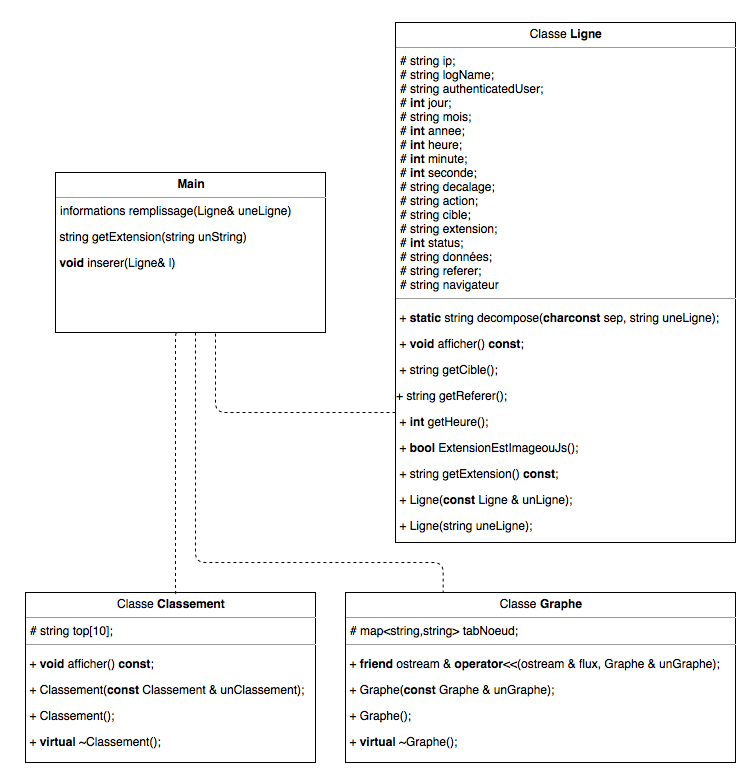
\includegraphics[scale=0.6]{diag.png} 
\end{center}
\caption{Diagramme de Classe}
\label{Diagramme de Classe}
\end{figure}
\end{section}


\begin{section}{Structures de données commentées et justifiées}
Au vu de la quantité de données à traiter, il est essentiel d'avoir la structure de données la plus adéquate possible, qui prenne le moins de place possible en mémoire pour que notre programme soit capable de s'exécuter rapidement et correctement. Pour cela il faut éviter le plus possible la redondance d'informations ainsi que le stockage d'informations inutiles.
Nous avons donc réfléchi à la manière de structurer les données avant de développer l'outil analog. Les principales données à organiser sont celles contenues dans la classe Ligne. Nous devions récupérer les informations qui nous étaient nécessaires dans une structure de données adéquate. Nous avons choisi d'utiliser le conteneur map de la STL.


Dans notre programme, les informations les plus importantes d'une ligne sont les attributs cible et referer. En effet, nous cherchons par défaut le nombre d'appel à un site cible. Avec l'option -g, il faut de plus connaître le nombre d'appel d'un site cible depuis un site referer particulier. Il nous semblait donc interessant de faire un premier map avec en clé le nom du site cible car celui ci est unique. Effectivement si l'on trouve dans notre fichier texte deux sites cibles identiques c'est que l'on parle du même et donc il faut prendre cela en compte au même endroit de notre map. C'est pour cela que nous avons liés à chaque clés une structure nommée informations que nous avons nous-même défini. 

Tout d'abord, on y retrouve le nombre de fois où la cible apparait dans le fichier. Cette valeur nous est indispensable pour pouvoir ensuite faire notre classement des 10 sites les plus visités. Nous avons choisis le type int car il est suffisant pour le jeu de données fourni mais si nécessaire il peut toujours être envisagé de l'étendre.
De plus, notre structure informations est aussi composée d'un conteneur map similaire à celui précédemment décrit puisqu'il prend en clé le nom des sites referers et en valeur le nombre de fois où le referer a cherché à accéder à la cible. C'est indispensable pour exécuter notre programme avec l'option -g car il faut connaitre le nombre de fois où un referer particulier appel une cible particulière.

C'est donc pour cela que nous avons choisi de faire ce conteneur map mapReferers dans la structure informations, elle-même valeur du conteneur map mapCibles car il nous est seulement utile de savoir combien de fois un referer apparait pour une cible précise.

Le conteneur map est global à l'ensemble de l'application, il obtenu dès le début à la lecture du fichier de logs fourni en paramètre. 

Avec cela, nous sommes donc capable de gérer notre classement des sites les plus visités de façon rapide car il n'y a pas de calcul à faire, nous avons juste à parcourir toutes les cibles de notre conteneur map et à prendre la cible ayant la plus grande valeur pour la variable iterations. Nous pouvons aussi générer notre fichier .dot de manière directe sans calcul supplémentaire en parcourant pour chaque cible tous les referers associés et y récupérer le nombre d'association entre les deux.
\newline

Une autre structure a été importante pour la conception de la classe Graphe. Le problème suivant s'est présenté : comme un site peut être à la fois une cible et un referer, il n'est pas suffisant de parcourir la map mapCibles et d'afficher toutes les clés, et pour chacune d'elles, toutes les clés du conteneur map mapReferers de la structure informations. Nous avons donc utilisé un autre conteneur map qui a pour clé un site (type string) et valeur associée un noeud du graphe (type string également). Ainsi, avant d'ajouter un nouveau noeud dans le fichier au format GraphViz, nous verifions qu'il n'est pas déjà présent dans le conteneur map attribut de la classe.




\end{section}

\end{document}
